\chapter{Fundamentação teórica} \label{chap:fundamentacao}

Este capítulo visa realizar uma abordagem de toda a fundamentação teórica e tecnológica necessária para o entendimento da solução proposta neste trabalho.

\section{\mqtt}

O \textit{Message Queue Telemetry Transport} (\mqtt)\footnote{\url{http://mqtt.org}} é um protocolo baseado em mensagens e seguindo o modelo \pubsub, utiliza o conceito de tópicos gerenciados por componentes chamados de \brokers. Originalmente projetado para o uso em redes não confiáveis e com recursos limitados, consiste em um servidor \broker e dois tipos distintos de clientes, \pubs e \subs \cite{lee:et-al:2013}.

O \broker funciona como um intermediador entre as mensagens que são enviadas por \pubs e recebidas por \subs. Toda a comunicação é feita por intermédio de tópicos, que funcionam como uma hierarquia de diretórios onde as mensagens são entregues. Os \pubs publicam mensagens no \broker em um determinado tópico, e este se encarrega de realizar a entrega da mensagem para os \subs que registraram interesse naquele tópico, fazendo com que a orquestração da comunicação entre as entidades produtoras e consumidoras de dados seja feita exclusivamente pelo \broker. O processo de entrega de mensagens pode ser visto na \autoref{fig:mqtt-sequence}.

\begin{figure}[htb]
	\caption{Diagrama de sequência do processo de entrega de mensagens no \mqtt}
	\label{fig:mqtt-sequence}
	\centering
	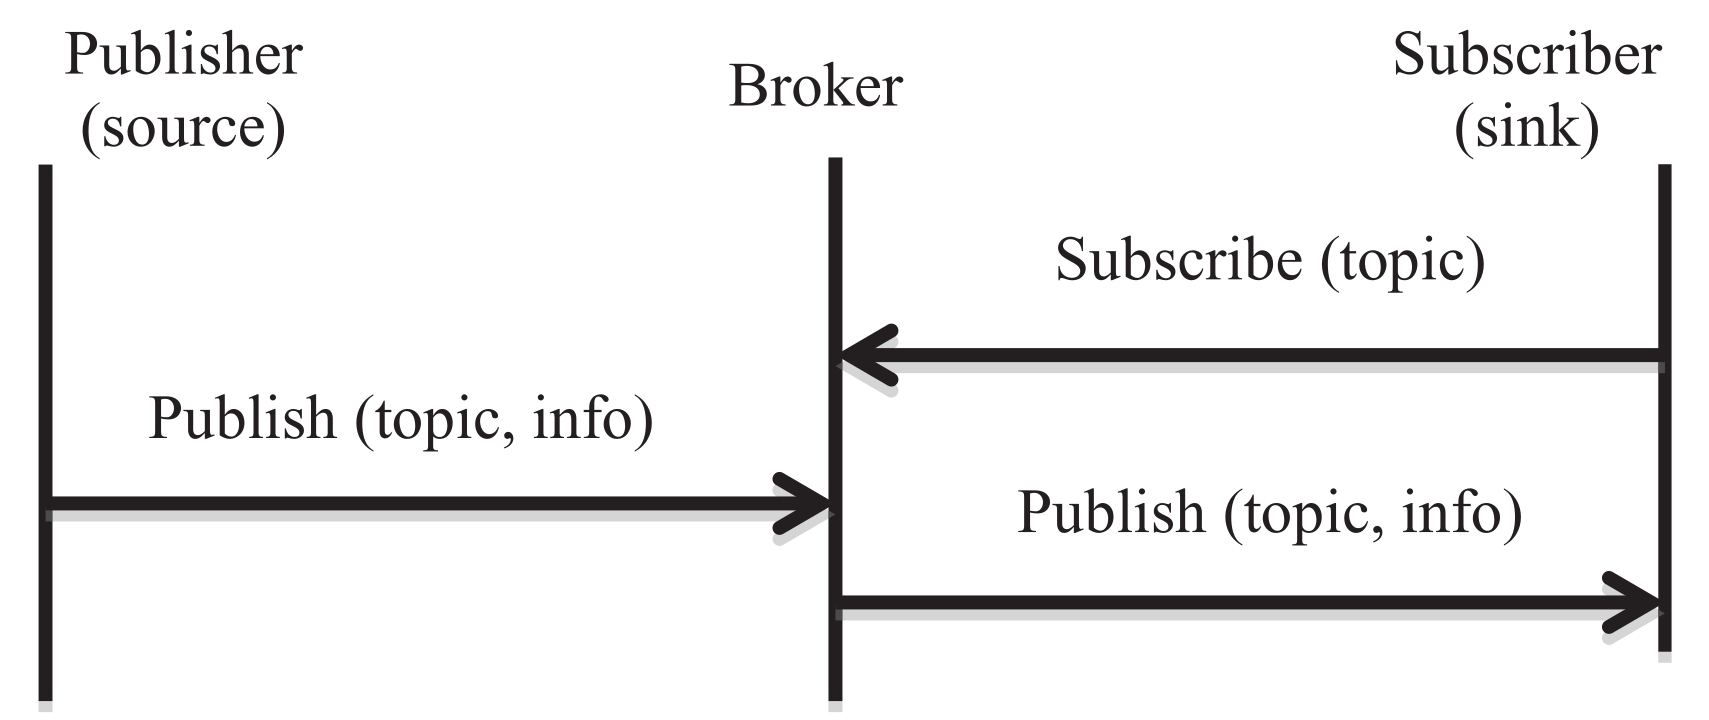
\includegraphics[width=0.85\linewidth]{img/mqtt-sequence.png}
	\fonte{\citeonline{al-fuqaha:et-al:2015}}
\end{figure}

Este protocolo permite o desacoplamento total entre os produtores e consumidores de dados, deste modo nenhum dos dois componentes têm ciência da existência mútua entre si.

\subsection{Estrutura de tópicos}

Existem dois elementos em uma mensagem \mqtt---o dado e o tópico. O dado é a informação que o \pub precisa enviar, este dado será então enviado para o \sub que assinou o tópico onde a mensagem foi publicada \cite{tantitharanukul:et-al:2017}.

O \pub pode definir qualquer tópico para enviar uma mensagem, com um ou mais níveis de hieraquía, cada nível é separado por uma barra (e.g., \texttt{thailand/humidity} ou \texttt{thailand/bangkok/traffic}).

Também existe a conveniência da utilização de caracteres coringas para a assinatura de tópicos, como por exemplo \texttt{thailand/+/traffic} onde o caractere ``\texttt{+}'' corresponde a qualquer padrão de um único nível de uma hierarquía, neste caso terceiro nível, podendo ser utilizado para receber os dados de tráfego de qualquer cidade da Tailândia. Outro caractere coringa que pode ser utilizado é o ``\texttt{\#}'' que corresponde a todos os níveis subsequentes de uma hierarquia, este só pode ser utilizado como o último caractere de uma subscrição \cite{hunkeler:truong:stanford-clark:2008}.

Dado o seguinte tópico \texttt{a/b/c/d}, as seguintes assinaturas irão receber os dados publicados nele \cite{light:mosquitto}:

\begin{alineas}
	\item \texttt{a/b/c/d};
	\item \texttt{\#};
	\item \texttt{a/\#};
	\item \texttt{a/b/\#};
	\item \texttt{a/b/c/\#};
	\item \texttt{+/b/c/\#}.
\end{alineas}

O \mqtt é o protocolo padrão utilizado pelo \cddl para realizar troca de mensagens entre diferentes componentes, como será discutido na \autoref{subsec:cddl}.
		
\section{\mhubcddl}

O \mhubcddl é uma composição de um \gateway (\mhub) e um \middleware de \iomt (\cddl). Enquanto o \mhub transforma o dispositivo \android em que está em execução em um \gateway \iot móvel, o \cddl funciona como \middleware provendo serviços locais e remotos de descoberta de provedores de serviços, processamento de eventos complexos, publicação e assinatura de dados e eventos com qualidade de serviço.

As seções seguintes abordarão cada um desses componentes separadamente.

\subsection{\mhub}

O \middleware \mhub pode ser definido, de acordo com \citeonline{talavera:et-al:2015}, como um serviço de \middleware de \iomt geral executado em um dispositivo móvel pessoal, responsável por descobrir e oportunisticamente conectar à uma miríade de \smartobjs acessíveis apenas através de tecnologias WPAN de curto alcance. Por estar envolvido com cenários de \iomt, este componenete de \software tem que lidar com situações que apresentam muito mais indeterminismo, devido à fatores como a menor garantia de disponibilidade de sensores e atuadores, confiabilidade reduzida, maior volatilidade em conexões, etc.

O \smartphone executando uma intância do \mhub, funciona como \gateway para \smartobjs, fornecendo acesso à Internet para dispositivos que não podem se conectar. Outro recurso importante que pode ser explorado pelas aplicações é a habilidade de enriquecer os dados de sensores com dados de contexto obtidos dos sensores internos do \mhub.

Para que o \mhub tenha suporte à determinada tecnologia de comunicação, é necessário que um novo módulo seja implementado. Este módulo será responsável por gerenciar quaisquer operações que sejam necessárias para garantir o funcionamento desta tecnologia.

\subsubsection{\stwopa} \label{subsub:s2pa}

Para gerenciar a descoberta e conexão com dispositivos que trabalham com diferentes tecnologias de comunicação, além dos sensores internos do \smartphone, o \mhub utiliza o \textit{Short-range Sensing, Presence \& Actuation} (\stwopa), um protocolo que fornece uma \api comum para realizar a comunicação com diferentes tecnologias WPAN.

Implementado como um módulo na arquitetura do \middleware, o \stwopa define um conjunto de métodos e interfaces que os módulos responsáveis por determinada tecnologia de comunicação devem implementar. Isto permite que o \stwopa se comunique com todas as tecnologias WPAN suportadas, gerenciando-as, e assim fornece uma \api unificada para todas as camadas superiores da arquitetura que precisam se comunicar com tais tecnologias.

O \stwopa torna-se então um intermediador entre todas as tecnologias de comunicação específicas e os demais componenetes do \middleware. Dentre as funcionalidades---na forma de métodos e interfaces---que as tecnologias devem implementar para seu correto funcionamento no \middleware, destacam-se:

\begin{alineas}
	\item descoberta e conexão de \smartobjs;
	
	\item descoberta de serviços de cada \smartobjs;

	\item leitura e escrita de atributos de serviços (\textit{e.g.}, dados de sensores e comandos de atuadores);

	\item notificação de desconexão com \smartobjs.
\end{alineas}

É possível encontrar na \autoref{fig:technology-interface} a interface \techinterface definida pelo \stwopa que declara os métodos padrões que realizam as funcionalidades descritas, a qual todas as tecnologias devem implementar. Também é ilustrada a interface \techlistener que é implementada pela classe \stwopaservice---a implementação do \stwopa no \mhub.

\begin{figure}[htb]
	\centering
	\caption{\label{fig:technology-interface}Interface \techinterface}
	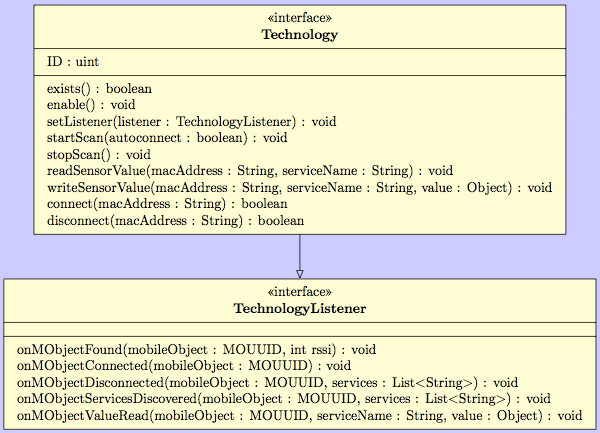
\includegraphics[scale=0.6]{img/technology-interface.png}
	\fonte{\citeonline[p.~125]{talavera:et-al:2015}}
\end{figure}

Além das tecnologias suportadas pelo \mhub, foi implementado uma pseudo tecnologia chamada de \faketechnology.
Esta não controla nenhuma tecnologia real, mas é interpretada como tal pelo \stwopa, seu objetivo é permitir geração de eventos de descoberta, conexão e desconexão no \stwopa a partir da camada de aplicação, não necessitando a presença de objetos físicos que se comuniquem em determinada WLAN.
Esta tecnologia foi utilizada para a realização das avaliações da solução proposta por este trabalho, como descrito no \autoref{chap:avaliacao}.

O \stwopaservice utiliza os métodos da interface \techinterface para gerenciar as tecnologias suportadas e, em particular, utiliza o método \texttt{setListener()} para se cadastrar como o \listener daquela tecnologia. Já as tecnologias utilizam os métodos da interface \techlistener para informar ao \stwopaservice a ocorrência de eventos com \smartobjs, como: descoberta, conexão, desconexão e leitura de dados de sensores.

Quando o \stwopaservice recebe de alguma tecnologia, um evento de descoberta, conexão, desconexão ou leitura de dados de \smartobjs, ele o ecapsula em um objeto do tipo \sensordata.
Esta classe possui os seguintes atributos:

\begin{alineas}
	\item \texttt{mouuid}: Uma combinação entre o \textit{id} da tecnologia que gerou tal evento com o endereço MAC do \smartobj;

	\item \texttt{signal}: Número em ponto flutuante onde o RSSI (\textit{Receiver Signal Strength}) daquela interação com o \smartobj é armazenado. O RSSI representa a intensidade de sinal naquele momento;

	\item \texttt{action}: Indica que tipo de evento uma instância de \sensordata está encapsulando. Os valores possíveis são as constantes:

	\begin{alineas}

		\item \texttt{FOUND}: Indica que um \smartobj foi descoberto pelo \mhub no ambiente;

		\item \texttt{CONNECTED}: Indica que o \mhub realizou uma conexão com o \smartobj;

		\item \texttt{READ}: Indica que uma leitura foi realizada, ou seja, o \smartobj enviou dados ao \mhub;

		\item \texttt{DISCONNECTED}: Indica que a conexão com o \smartobj foi desfeita.

	\end{alineas}

	\item \texttt{sensorName}: Representa o nome do \smartobj;

	\item \texttt{sensorValue}: Um vetor de pontos flutuantes que armazena os valores lidos do \smartobj. Logicamente este atributo só possui valores quando o atributo \texttt{action} assume o valor \texttt{READ}.
\end{alineas}

O \mhub fornece diversos serviços que não serão tratados neste trabalho, dentre eles, destaca-se \cite{gomes:2017}:

\begin{alineas}
	\item \emph{protocolo de transcodificação}:
		Os pacotes de dados recebidos dos sensores podem ter diferentes formatos e codificações.  Assim, o \mhub deve transcodificá-los e serializá-los, antes de transmiti-los. A transcodificação de dados é altamente dependente do tipo, marca e fabricante do sensor;
		
	\item \emph{caching de dados}:
		A fim de otimizar a transmissão para a nuvem através da Internet móvel, o \mhub pode agrupar várias amostras de dados obtidas a partir de vários sensores próximos antes de enviá-las ao gateway em rajada única. Para isso, o \mhub armazena em cache as amostras de dados recebidas dos sensores;
		
	\item \emph{configuração e controle dos sensores}:
		Dependendo do tipo de sensor, o \mhub pode, eventualmente ou periodicamente, enviar comandos, definições de parâmetros ou requisições de consultas de dados através da WPAN para os sensores conectados;
		
	\item \emph{pré-processamento de dados do sensor}:
		Antes de enviar os dados, pode ser necessário aplicar uma função de pré-processamento (e.g.  transcodificação, formatação, agregação, filtragem, ou comparação com leituras anteriores etc.).  Esse pré-processamento é feito no \mhub;
		
	\item \emph{carregamento dinâmico de módulos do sensor}:
		Uma vez que não é possível ter módulos internos para todos os sensores que podem estar disponíveis a medida que o gateway se move, o \mhub oferece um mecanismo de implantação de módulo em tempo de execução e gerenciamento do ciclo de vida desses módulos;
		
	\item \emph{processamento nas pontas}:
		O \mhub oferece mecanismos que permitem aos desenvolvedores de aplicações distribuírem as funcionalidades do seu código entre o dispositivo móvel e nodos da nuvem, movendo parte do processamento das informações de contexto para “as pontas” do sistema. A isso se dá o nome de In-Network Processing, uma técnica que ajuda a diminuir a quantidade de informações a ser transmitida para a nuvem, podendo melhorar a escalabilidade do sistema. O processamento ao qual esta funcionalidade se refere pode ser implementado em código Java convencional ou utilizando EPL Esper;
		
	\item \emph{processamento ciente de energia}:
		Por meio de um componente de gerenciamento de energia, o \mhub monitora o nível da bateria do dispositivo móvel, disparando ações adaptativas que ajustam os comportamento dos seus serviços, de acordo com a disponibilidade de energia do dispositivo móvel. Por exemplo, a frequência de publicação dos dados por ser reduzida quando o nível da bateria está baixo (por exemplo, menor que 20\%).
\end{alineas}

A arquitetura do \middleware pode ser observada na \autoref{fig:m-hub-architecture}.

\begin{figure}[htb]
	\centering
	\caption{\label{fig:m-hub-architecture}Arquitetura do \mhub}
	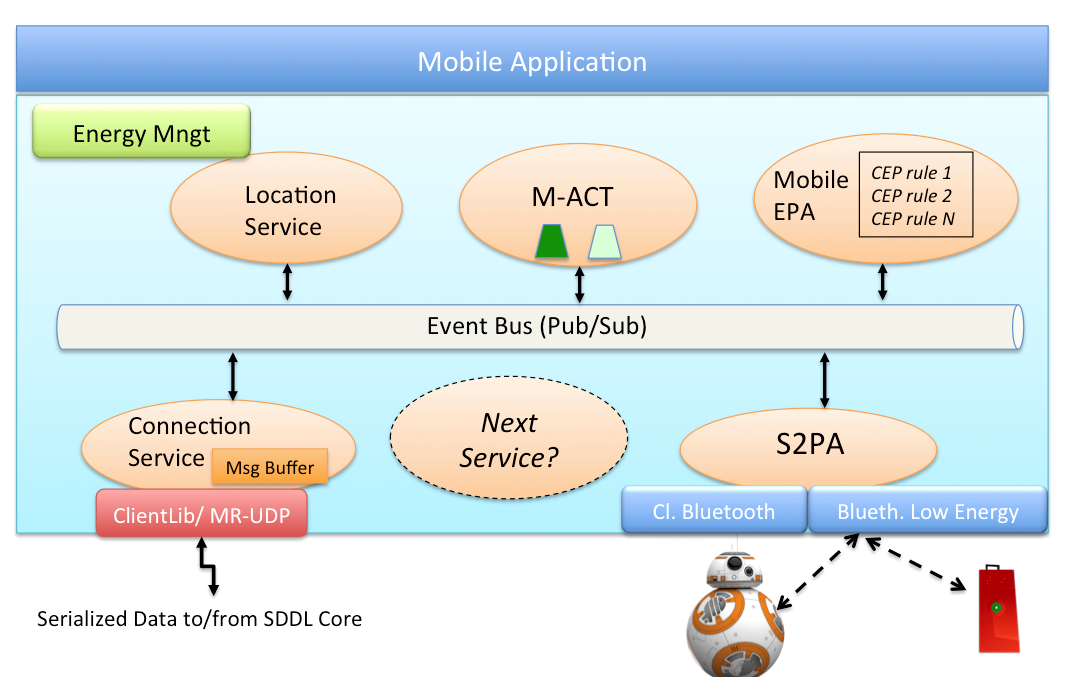
\includegraphics[scale=0.34]{img/m-hub-architecture.png}
	\fonte{\citeonline[p.~6]{endler:silva:2018}}
\end{figure}

\subsection{\cddl} \label{subsec:cddl}

O \cddl é uma camada de distribuição de dados que provê mecanismos que permitem a especificação, controle e monitoramento de requisitos de qualidade de informação e do serviço de distribuição de dados \cite{gomes:2017}.

A interação entre produtores e consumidores de dados de contexto se dá através do modelo \pubsub com a utilização de \brokers, implementando uma comunicação ditribuída com o \mqtt. O \cddl também fornece um \ubroker que executa internamente no dispositivo móvel, o que permite que certas aplicações possam publicar e receber dados sem a dependência de conexão à Internet.

Todos os dados que são publicados pelo \cddl são instâncias da classe \msg.
Esta classe encapsula diversos atributos relevantes aos dados de contexto que representam, dentre eles, destaca-se:

\begin{alineas}
	\item \texttt{serviceName}: Nome do \smartobj que está relacionado a essa \msg;

	\item \texttt{serviceValue}: Valor da leitura dos dados do \smartobj;

	\item \texttt{accuracy}: Acurácia do dado;

	\item \texttt{measurementTime}: O \timestamp em que a \msg foi gerada;

	\item \texttt{sourceLocationLatitude}: Latitude do \mhub que gerou este dado;

	\item \texttt{sourceLocationLongitude}: Longitude do \mhub que gerou este dado;

	\item \texttt{sourceLocationAltitude}: Altitude do \mhub que gerou este dado;

	\item \texttt{signal}: Intensidade do sinal no momento em que o \smartobj interagiu com o \stwopa.
\end{alineas}

Como ja mencionado, o modelo de programação do \cddl respeita o padrão \pubsub, então uma aplicação que registra o interesse por algum tipo de dado de contexto será notificada através de um objeto \msg, que representa este dado.
O \autoref{lst:subscriber} apresenta um exemplo de como o desenvolvedor pode consumir dados de temperatura capturados pelo \middleware.

\lstinputlisting[float=htb,label=lst:subscriber, caption=Modelo de programação \pubsub do \cddl]{code/Subscriber.java}

Como \middleware, o \cddl permite que as aplicações clientes assumam o papel de produtoras ou consumidoras de dados de contexto, fornecendo suporte à políticas de qualidade de serviço de distribuição de dados. Desta forma as aplicações podem especificar parâmetros que expressam seus requisitos de QoC para envio e recebimento de mensagens. A fim de fornecer suporte para o desenvolvimento de aplicações de \iot e \iomt, o \cddl atende aos seguintes requisitos \cite{muniz:2017}:

\begin{alineas}
	\item suporte à distribuição de dados local e remota;

	\item suporte ao registro e descoberta distribuída de serviços;

	\item modelo de programação uniforme e independente de localização;

	\item suporte à entrega confiável de dados em cenários de mobilidade;

	\item provisionamento e monitoramento de qualidade da informação;

	\item provisionamento e monitoramento de qualidade do serviço de distribuição;

	\item filtragem das informações.
\end{alineas}

\subsection*{O \middleware \mhubcddl}

O \mhubcddl é uma abordagem de \middleware para desenvolvimento de aplicações de \iomt e \iot, utiliza o \mhub como o componente responsável pela descoberta e aquisição dos dados diretamente dos \smartobjs, abstraindo especificidades de comunicação de suas WPANs. O \cddl foi escolhido como a camada de distribuição de dados, que provê o controle de requisitos de qualidade de informação e fornce uma \api única.

A \autoref{fig:mhub-cdll-architecture} ilustra a arquitetura do \middleware.
O \mhub funcionando como \gateway móvel entre os \smartobjs e a Internet, tranferindo ao \cddl os dados de contexto capturados através do \eventbus.
Uma vez entregue ao \cddl, todos os dados são então publicados em uma estrutura de tópicos de um \broker \mqtt, local ou não.
Desta forma sendo entregue às aplicações que registraram no \broker interesse em tais dados.

\begin{figure}[htb]
	\centering
	\caption{\label{fig:mhub-cdll-architecture}Arquitetura do \mhubcddl}
	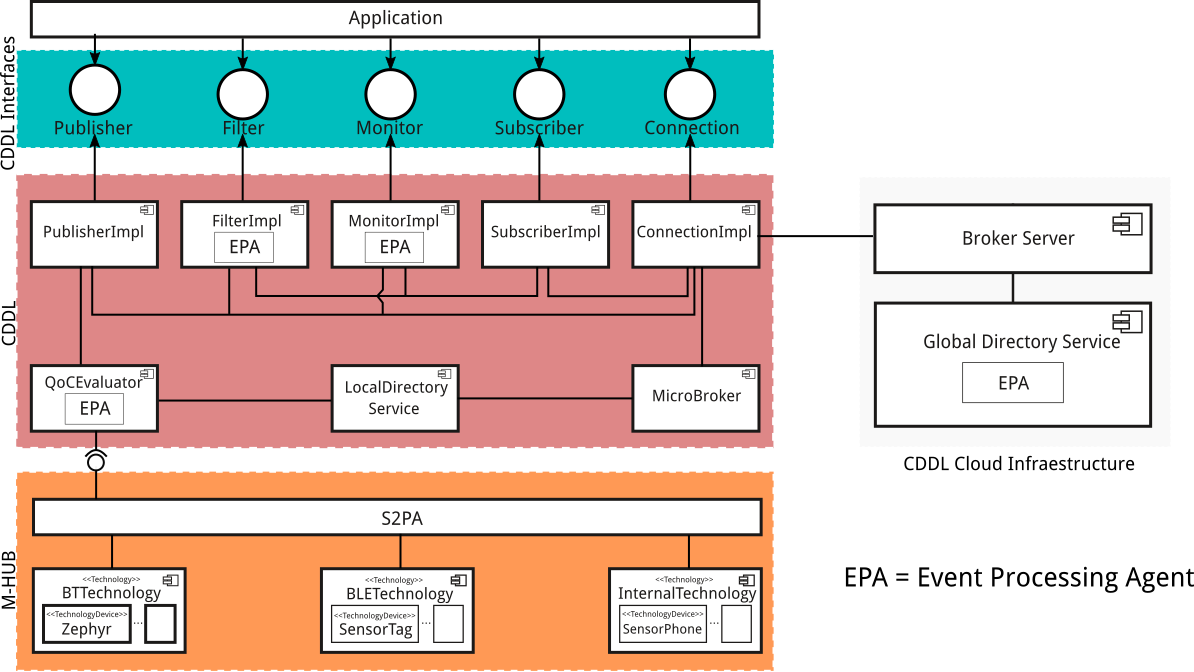
\includegraphics[width=0.85\linewidth]{img/mhub-cddl-architecture.png}
	\fonte{\citeonline[p.~15]{gomes:et-al:2017}}
\end{figure}

